\documentclass[a4paper,12pt]{report}

\usepackage{setspace}
\onehalfspacing

\usepackage{anysize}
\marginsize{2cm}{2cm}{2cm}{2cm}

\usepackage{graphicx}
\usepackage{caption}
\usepackage[utf8]{inputenc}

\usepackage{csquotes}
\usepackage[australian]{babel}

\usepackage[backend=biber]{biblatex}
\addbibresource{thesis.bib}

\usepackage{hyperref}

\usepackage{pgfplots}
\pgfplotsset{width=\textwidth,compat=1.9}

\usepgfplotslibrary{external}
\tikzexternalize

\author{Lasath Fernando}
\title{Thesis A}
\date{15/10/14}

\begin{document}
\maketitle


\chapter{Introduction}
\section{Combination Process}
\section{Hidden Markov Models}
\section{iHMMuneAlign}
Developed in 2007 by a team of researchers at UNSW, iHMMuneAlign attempts to simulate this process \autocite{iHMMuneAlign}.
It represents the combination process of immunoglobulin heavy chain genes as a hidden markov model.


\chapter{Analysis}
Since the high level aim of this project is to improve the performance of iHMMuneAlign, it was necessary to analyze the existing implementation in order to gain insight into its structure, as well as to create realistic aims. 

\section{Run Time}
One of the primary attributes of performance, is run time. We begin by measuring the run time of the existing implementation and -more importantly- how it grows with workload.

The current implementation consists of a Java executable and a shell script, to allow running in batches. The Java executable (which does the actual processing) takes a range of input from the script and attempts to process that many in paralell. It then invokes Java program after breaking up the entire range into batches of a given size.

Since we are interested in the rate the total runtime changes with workload as well with increasing paralellism, both were measured. It was run with a total workload ranging from 1 sequences to 100 sequences, with batch size ranging from 1 to 8. The results are shown in \autoref{fig:runtime}.

%TODO: describe machine specs

\subsection{Interpretation of Results}
With a batch size of 1, the expected linear increase was present. However, increasing the batch size shows a more sporadic decrease in runtime. This is to be expected, since concurrent programs tend to be very non-deterministic in execution time. However, there is an overall decrease in total execution time, as the batch size increases.

%% TODO: replace jit reference with paper from IBM
While this is in part due to the parallel nature of the existing implementation, it is also due to the overhead from invoking the Java program reducing. In each invocation, the Java Virtual Machine (JVM) has to be created, the program loaded (and JIT compiled \autocite{jit}), and the program itself needs to read the repitoire files etc. Since all this only has to be done once per batch, reducing the number of batches also reduced the total work needed to be done significantly. This can be seen in \autoref{fig:usertime}, which shows that the CPU time (total time that all the CPUs spent working, rather than waiting for each other, and waiting for disk/system operations) also reduces with batch size.

\begin{figure}[h]
  \centering
  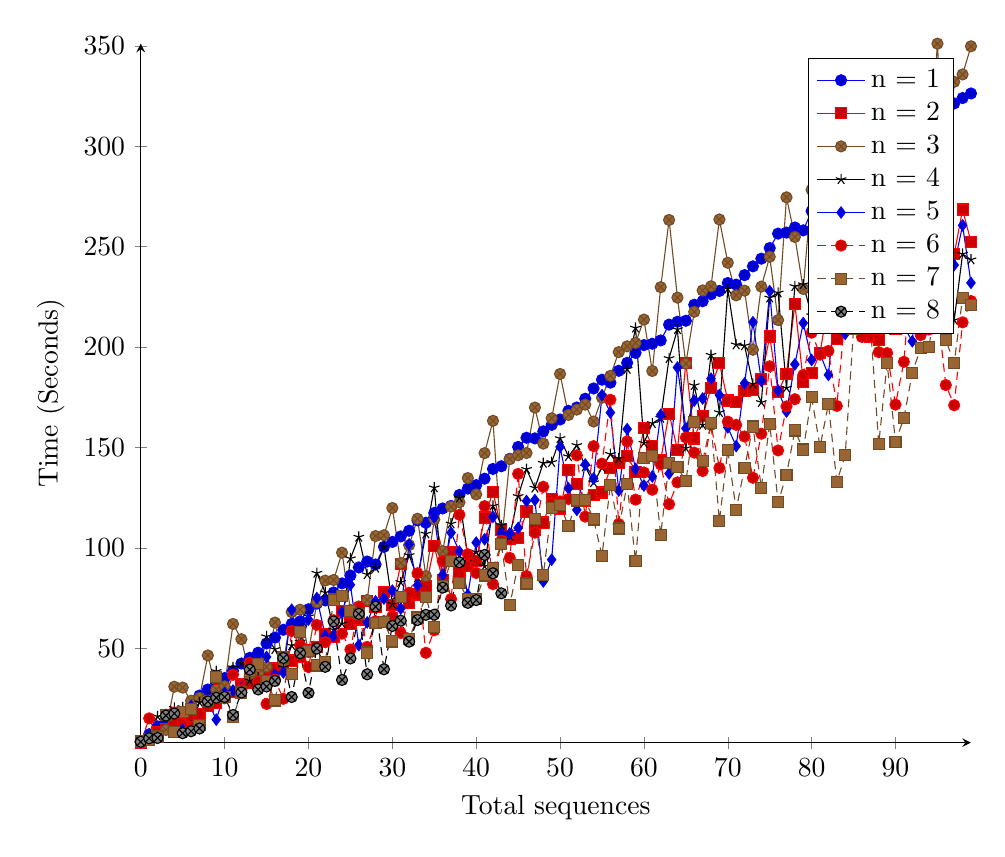
\begin{tikzpicture}
    \begin{axis}[
      axis lines = left,
      xlabel = Total sequences,
      ylabel = Time (Seconds),
    ]

      \addplot coordinates {(0, 3.666) (1, 7.209) (2, 11.098) (3, 13.184) (4, 17.882) (5, 18.165) (6, 21.92) (7, 26.444) (8, 29.46) (9, 32.378) (10, 35.191) (11, 38.779) (12, 42.411) (13, 45.237) (14, 47.817) (15, 52.443) (16, 55.323) (17, 59.223) (18, 62.145) (19, 63.403999999999996) (20, 69.451) (21, 72.27) (22, 73.858) (23, 77.786) (24, 82.32) (25, 86.237) (26, 90.262) (27, 93.215) (28, 91.743) (29, 100.52600000000001) (30, 102.97800000000001) (31, 105.72399999999999) (32, 108.535) (33, 113.708) (34, 112.515) (35, 117.419) (36, 119.632) (37, 120.91) (38, 126.353) (39, 129.523) (40, 131.26) (41, 134.462) (42, 139.297) (43, 140.651) (44, 144.345) (45, 150.274) (46, 154.83100000000002) (47, 154.53) (48, 158.02) (49, 161.261) (50, 163.946) (51, 168.232) (52, 169.903) (53, 174.255) (54, 179.395) (55, 183.74) (56, 182.267) (57, 188.184) (58, 192.145) (59, 197.113) (60, 200.958) (61, 201.651) (62, 203.308) (63, 211.17000000000002) (64, 212.591) (65, 213.102) (66, 221.066) (67, 222.832) (68, 226.29) (69, 227.94) (70, 231.871) (71, 231.076) (72, 235.82) (73, 240.191) (74, 244.004) (75, 249.306) (76, 256.481) (77, 256.99) (78, 259.532) (79, 258.101) (80, 267.729) (81, 268.332) (82, 269.785) (83, 273.914) (84, 281.647) (85, 280.175) (86, 280.546) (87, 288.436) (88, 295.22) (89, 300.093) (90, 300.374) (91, 300.545) (92, 302.711) (93, 311.689) (94, 311.437) (95, 313.11) (96, 318.581) (97, 321.303) (98, 323.983) (99, 326.274)};
\addlegendentry{n = 1}
\addplot coordinates {(0, 3.08) (1, 4.869) (2, 8.224) (3, 9.747) (4, 13.009) (5, 12.466) (6, 16.181) (7, 17.423) (8, 21.338) (9, 22.92) (10, 26.964) (11, 28.107) (12, 31.971) (13, 32.888) (14, 34.992) (15, 38.017) (16, 39.936) (17, 42.365) (18, 43.898) (19, 45.748) (20, 48.998) (21, 50.76) (22, 56.908) (23, 55.468) (24, 68.413) (25, 62.305) (26, 64.368) (27, 73.522) (28, 70.631) (29, 78.002) (30, 71.632) (31, 92.09700000000001) (32, 72.732) (33, 76.798) (34, 80.75) (35, 100.762) (36, 83.911) (37, 97.86699999999999) (38, 87.968) (39, 91.15899999999999) (40, 93.555) (41, 115.116) (42, 127.925) (43, 109.143) (44, 104.608) (45, 104.844) (46, 118.08) (47, 108.715) (48, 112.625) (49, 124.212) (50, 119.345) (51, 138.649) (52, 131.713) (53, 123.5) (54, 126.269) (55, 127.579) (56, 139.672) (57, 142.149) (58, 145.877) (59, 137.982) (60, 159.735) (61, 150.606) (62, 143.906) (63, 166.844) (64, 148.841) (65, 192.249) (66, 154.497) (67, 165.55) (68, 179.69299999999998) (69, 191.857) (70, 173.351) (71, 172.472) (72, 178.026) (73, 178.61) (74, 184.22) (75, 205.282) (76, 177.747) (77, 186.55) (78, 221.452) (79, 182.756) (80, 186.925) (81, 197.087) (82, 221.88) (83, 204.239) (84, 231.477) (85, 218.072) (86, 219.494) (87, 204.859) (88, 203.554) (89, 215.624) (90, 208.877) (91, 252.853) (92, 246.432) (93, 236.011) (94, 219.126) (95, 252.926) (96, 233.982) (97, 246.214) (98, 268.499) (99, 252.289)};
\addlegendentry{n = 2}
\addplot coordinates {(0, 3.559) (1, 4.559) (2, 5.687) (3, 9.354) (4, 30.875) (5, 30.426) (6, 23.9) (7, 25.339) (8, 46.432) (9, 29.46) (10, 31.107) (11, 62.127) (12, 54.525) (13, 36.189) (14, 37.487) (15, 40.764) (16, 62.808) (17, 42.793) (18, 68.037) (19, 69.226) (20, 48.114) (21, 72.818) (22, 83.715) (23, 84.009) (24, 97.636) (25, 69.094) (26, 70.809) (27, 74.071) (28, 105.88900000000001) (29, 106.28) (30, 119.86699999999999) (31, 92.483) (32, 101.376) (33, 114.50200000000001) (34, 85.971) (35, 114.10900000000001) (36, 98.32) (37, 120.58) (38, 122.655) (39, 134.764) (40, 126.619) (41, 147.17000000000002) (42, 163.27100000000002) (43, 101.68) (44, 144.171) (45, 146.132) (46, 147.236) (47, 169.875) (48, 151.916) (49, 164.513) (50, 186.606) (51, 166.211) (52, 168.836) (53, 171.339) (54, 162.90699999999998) (55, 174.773) (56, 185.661) (57, 197.483) (58, 200.379) (59, 202.04) (60, 213.675) (61, 188.085) (62, 229.81) (63, 263.275) (64, 224.61) (65, 191.714) (66, 217.549) (67, 228.19299999999998) (68, 230.237) (69, 263.532) (70, 241.97) (71, 225.755) (72, 228.06900000000002) (73, 198.656) (74, 230.089) (75, 244.961) (76, 213.415) (77, 274.54) (78, 254.812) (79, 228.93) (80, 278.3) (81, 294.204) (82, 254.605) (83, 320.259) (84, 258.843) (85, 251.48) (86, 272.09000000000003) (87, 287.05) (88, 297.918) (89, 261.177) (90, 250.419) (91, 293.244) (92, 282.259) (93, 297.56) (94, 290.209) (95, 351.065) (96, 269.916) (97, 332.071) (98, 335.749) (99, 349.758)};
\addlegendentry{n = 3}
\addplot coordinates {(0, 3.419) (1, 4.882) (2, 16.053) (3, 16.885) (4, 20.265) (5, 20.597) (6, 11.26) (7, 23.028) (8, 25.691) (9, 38.561) (10, 27.902) (11, 40.432) (12, 42.566) (13, 33.868) (14, 35.53) (15, 55.869) (16, 49.503) (17, 40.467) (18, 51.354) (19, 53.217) (20, 65.789) (21, 87.471) (22, 77.72) (23, 59.246) (24, 62.274) (25, 94.709) (26, 105.422) (27, 86.739) (28, 89.992) (29, 100.52000000000001) (30, 72.056) (31, 82.867) (32, 96.285) (33, 85.206) (34, 107.005) (35, 129.983) (36, 81.316) (37, 112.021) (38, 124.889) (39, 95.654) (40, 97.937) (41, 90.809) (42, 120.868) (43, 111.219) (44, 105.894) (45, 125.689) (46, 139.176) (47, 129.849) (48, 142.207) (49, 142.641) (50, 154.536) (51, 145.52100000000002) (52, 151.07999999999998) (53, 140.382) (54, 132.532) (55, 139.877) (56, 146.661) (57, 144.443) (58, 189.001) (59, 209.526) (60, 152.183) (61, 161.983) (62, 164.647) (63, 194.393) (64, 208.77) (65, 149.619) (66, 180.88) (67, 161.16) (68, 195.997) (69, 167.473) (70, 228.893) (71, 201.182) (72, 200.731) (73, 181.622) (74, 172.48) (75, 224.528) (76, 227.016) (77, 179.654) (78, 230.243) (79, 231.126) (80, 215.712) (81, 227.744) (82, 235.21800000000002) (83, 248.569) (84, 240.358) (85, 263.79) (86, 254.481) (87, 274.367) (88, 237.482) (89, 270.356) (90, 261.882) (91, 222.9) (92, 225.739) (93, 287.957) (94, 235.978) (95, 258.283) (96, 262.224) (97, 213.429) (98, 246.329) (99, 243.495)};
\addlegendentry{n = 4}
\addplot coordinates {(0, 3.029) (1, 4.397) (2, 5.72) (3, 16.412) (4, 17.876) (5, 9.435) (6, 21.329) (7, 12.567) (8, 23.844) (9, 14.476) (10, 27.684) (11, 28.977) (12, 30.059) (13, 42.228) (14, 42.362) (15, 45.702) (16, 36.748) (17, 37.954) (18, 69.226) (19, 50.777) (20, 64.30199999999999) (21, 75.001) (22, 56.241) (23, 56.201) (24, 67.915) (25, 81.63) (26, 51.561) (27, 62.878) (28, 73.346) (29, 74.751) (30, 78.731) (31, 69.775) (32, 101.76599999999999) (33, 81.393) (34, 112.16499999999999) (35, 115.209) (36, 86.555) (37, 107.56700000000001) (38, 98.142) (39, 76.562) (40, 102.642) (41, 104.26599999999999) (42, 115.428) (43, 107.321) (44, 107.143) (45, 109.922) (46, 123.366) (47, 123.811) (48, 83.277) (49, 94.12100000000001) (50, 150.279) (51, 129.647) (52, 118.919) (53, 141.534) (54, 134.589) (55, 176.042) (56, 167.385) (57, 128.568) (58, 159.117) (59, 139.313) (60, 131.072) (61, 135.553) (62, 166.228) (63, 137.027) (64, 189.851) (65, 159.51) (66, 173.321) (67, 174.382) (68, 184.252) (69, 176.086) (70, 159.999) (71, 150.671) (72, 181.951) (73, 212.381) (74, 183.158) (75, 227.859) (76, 178.382) (77, 167.859) (78, 191.393) (79, 211.974) (80, 193.557) (81, 196.574) (82, 186.138) (83, 229.11) (84, 206.567) (85, 215.037) (86, 215.285) (87, 215.32) (88, 226.553) (89, 218.748) (90, 239.55700000000002) (91, 209.981) (92, 202.868) (93, 250.999) (94, 213.5) (95, 229.523) (96, 249.79) (97, 240.834) (98, 260.608) (99, 231.959)};
\addlegendentry{n = 5}
\addplot coordinates {(0, 3.056) (1, 15.12) (2, 5.714) (3, 16.867) (4, 17.973) (5, 17.85) (6, 10.673) (7, 12.224) (8, 23.858) (9, 34.538) (10, 25.095) (11, 36.827) (12, 29.27) (13, 42.836) (14, 33.381) (15, 22.295) (16, 34.439) (17, 24.841) (18, 58.569) (19, 51.43) (20, 40.647) (21, 61.67) (22, 53.047) (23, 63.963) (24, 57.297) (25, 49.378) (26, 70.59) (27, 50.655) (28, 63.471000000000004) (29, 63.497) (30, 65.935) (31, 57.617) (32, 77.62) (33, 87.384) (34, 47.759) (35, 58.975) (36, 93.417) (37, 74.533) (38, 116.485) (39, 96.848) (40, 87.498) (41, 120.783) (42, 81.94800000000001) (43, 103.559) (44, 95.02799999999999) (45, 136.82999999999998) (46, 85.974) (47, 107.57) (48, 130.437) (49, 122.401) (50, 123.129) (51, 124.351) (52, 146.085) (53, 115.57900000000001) (54, 150.674) (55, 141.938) (56, 173.764) (57, 111.89) (58, 153.006) (59, 124.029) (60, 137.536) (61, 128.934) (62, 141.599) (63, 121.761) (64, 132.622) (65, 154.93) (66, 147.444) (67, 138.28300000000002) (68, 161.327) (69, 139.817) (70, 162.856) (71, 161.25) (72, 155.465) (73, 134.902) (74, 156.853) (75, 190.429) (76, 148.512) (77, 170.463) (78, 174.029) (79, 186.058) (80, 207.168) (81, 196.221) (82, 198.037) (83, 170.688) (84, 215.75900000000001) (85, 225.70499999999998) (86, 205.029) (87, 226.43) (88, 197.476) (89, 197.006) (90, 171.336) (91, 192.656) (92, 244.355) (93, 205.919) (94, 208.721) (95, 218.261) (96, 181.074) (97, 171.026) (98, 212.301) (99, 222.90800000000002)};
\addlegendentry{n = 6}
\addplot coordinates {(0, 3.569) (1, 4.383) (2, 6.07) (3, 16.676) (4, 8.137) (5, 18.113) (6, 19.84) (7, 11.693) (8, 23.689) (9, 35.758) (10, 25.552) (11, 15.82) (12, 27.963) (13, 38.846) (14, 42.368) (15, 33.883) (16, 24.045) (17, 45.389) (18, 37.181) (19, 58.019) (20, 48.574) (21, 41.451) (22, 43.228) (23, 74.275) (24, 75.971) (25, 68.67699999999999) (26, 67.022) (27, 47.865) (28, 62.628) (29, 63.128) (30, 53.42) (31, 75.41) (32, 54.698) (33, 65.344) (34, 75.614) (35, 60.81) (36, 81.09700000000001) (37, 93.315) (38, 82.635) (39, 74.30799999999999) (40, 74.67) (41, 86.265) (42, 90.151) (43, 101.97) (44, 71.446) (45, 91.59100000000001) (46, 82.27) (47, 114.428) (48, 86.564) (49, 119.836) (50, 121.401) (51, 110.888) (52, 123.606) (53, 123.858) (54, 114.157) (55, 96.12899999999999) (56, 131.416) (57, 109.64699999999999) (58, 131.61599999999999) (59, 93.357) (60, 144.865) (61, 145.701) (62, 106.419) (63, 142.256) (64, 140.423) (65, 133.113) (66, 162.606) (67, 143.272) (68, 162.067) (69, 113.39) (70, 148.581) (71, 118.981) (72, 139.88) (73, 160.425) (74, 129.953) (75, 161.867) (76, 122.651) (77, 136.459) (78, 158.474) (79, 148.948) (80, 175.078) (81, 150.316) (82, 171.688) (83, 132.864) (84, 146.125) (85, 208.936) (86, 209.704) (87, 211.531) (88, 151.739) (89, 191.99099999999999) (90, 152.88) (91, 164.515) (92, 187.205) (93, 199.451) (94, 199.889) (95, 231.937) (96, 203.394) (97, 192.155) (98, 224.514) (99, 220.881)};
\addlegendentry{n = 7}
\addplot coordinates {(0, 3.442) (1, 5.184) (2, 5.343) (3, 16.489) (4, 17.528) (5, 7.724) (6, 8.69) (7, 10.07) (8, 23.518) (9, 25.375) (10, 25.766) (11, 16.758) (12, 27.975) (13, 39.373) (14, 29.487) (15, 30.963) (16, 33.746) (17, 45.191) (18, 25.746) (19, 47.603) (20, 27.751) (21, 49.86) (22, 40.769) (23, 63.373) (24, 34.238) (25, 44.943) (26, 67.144) (27, 37.029) (28, 70.723) (29, 39.537) (30, 61.086) (31, 63.739) (32, 53.315) (33, 64.053) (34, 66.66) (35, 66.749) (36, 80.206) (37, 71.322) (38, 92.846) (39, 72.612) (40, 74.006) (41, 96.497) (42, 87.361) (43, 77.36)};
\addlegendentry{n = 8}

    \end{axis}
  \end{tikzpicture}
  \caption{Total execution time (in seconds) to process the number of sequences. $n$ is the number of sequences per invocation of the program}
  \label{fig:runtime}
\end{figure}

\begin{figure}[h]
  \centering
  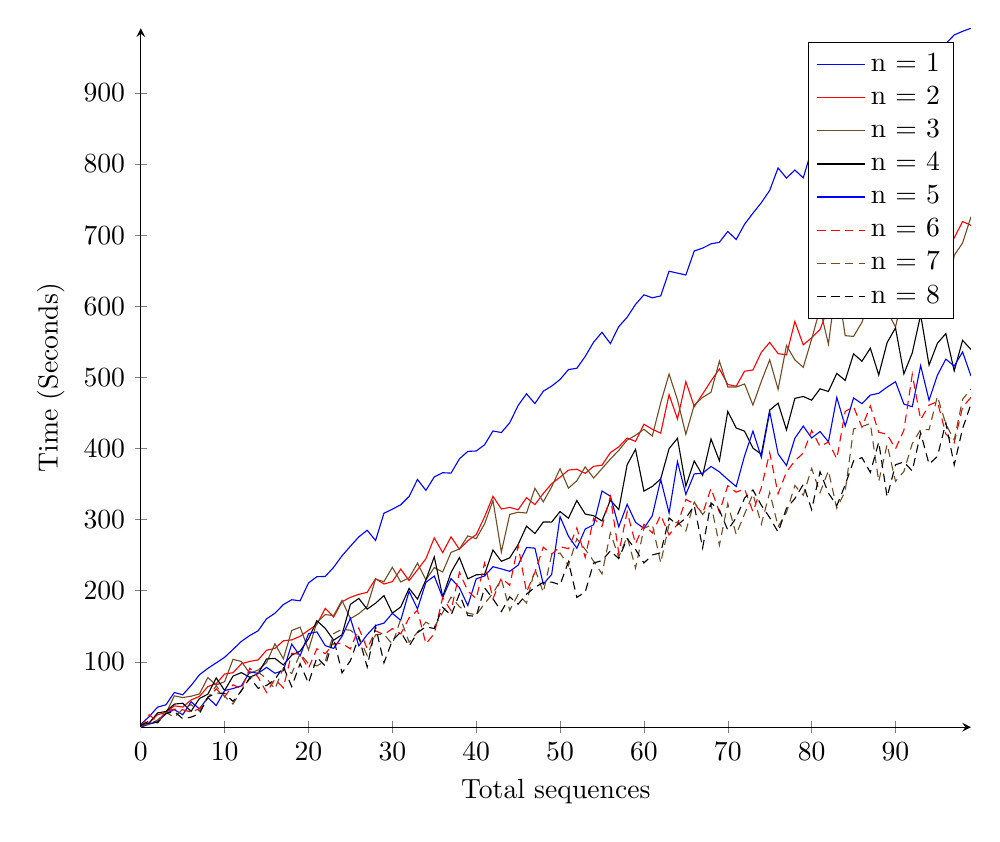
\begin{tikzpicture}
    \begin{axis}[
      axis lines = left,
      xlabel = Total sequences,
      ylabel = Time (Seconds),
    ]

      \addplot +[mark=none] coordinates {(0, 12.217) (1, 22.953) (2, 36.363) (3, 39.593) (4, 56.95) (5, 53.69) (6, 66.68299999999999) (7, 81.873) (8, 90.867) (9, 98.613) (10, 106.4) (11, 117.517) (12, 128.83) (13, 137.047) (14, 143.703) (15, 160.553) (16, 168.377) (17, 180.477) (18, 187.363) (19, 185.833) (20, 210.883) (21, 219.71699999999998) (22, 220.13) (23, 232.94) (24, 249.157) (25, 262.58) (26, 275.7) (27, 285.027) (28, 270.68) (29, 308.963) (30, 314.687) (31, 320.873) (32, 332.613) (33, 356.477) (34, 341.09000000000003) (35, 360.003) (36, 365.943) (37, 365.387) (38, 385.39300000000003) (39, 395.933) (40, 396.477) (41, 405.25) (42, 424.597) (43, 422.443) (44, 436.16700000000003) (45, 460.503) (46, 476.877) (47, 463.137) (48, 480.507) (49, 487.743) (50, 497.067) (51, 511.003) (52, 512.73) (53, 529.41) (54, 549.517) (55, 563.347) (56, 547.543) (57, 571.413) (58, 584.523) (59, 602.627) (60, 616.06) (61, 611.88) (62, 614.48) (63, 649.237) (64, 646.577) (65, 643.893) (66, 677.667) (67, 681.787) (68, 687.717) (69, 689.95) (70, 705.2) (71, 693.857) (72, 715.217) (73, 730.85) (74, 745.593) (75, 762.927) (76, 794.46) (77, 780.163) (78, 791.54) (79, 780.433) (80, 819.9) (81, 819.49) (82, 813.703) (83, 823.697) (84, 866.76) (85, 856.563) (86, 845.58) (87, 879.407) (88, 909.97) (89, 925.833) (90, 921.067) (91, 912.287) (92, 918.253) (93, 962.357) (94, 948.447) (95, 953.217) (96, 969.237) (97, 981.413) (98, 986.54) (99, 990.897)};
\addlegendentry{n = 1}
\addplot +[mark=none] coordinates {(0, 8.7) (1, 14.503) (2, 25.713) (3, 28.793) (4, 38.187) (5, 36.447) (6, 46.453) (7, 51.43) (8, 65.233) (9, 69.39) (10, 82.887) (11, 84.777) (12, 97.303) (13, 100.703) (14, 102.743) (15, 116.34) (16, 118.917) (17, 129.63) (18, 130.887) (19, 135.963) (20, 144.46) (21, 152.637) (22, 175.25) (23, 163.117) (24, 184.617) (25, 190.71) (26, 194.923) (27, 197.757) (28, 216.973) (29, 209.463) (30, 212.79) (31, 230.393) (32, 214.26) (33, 229.447) (34, 244.95) (35, 274.413) (36, 253.57) (37, 275.78) (38, 258.31) (39, 270.367) (40, 278.867) (41, 304.047) (42, 332.837) (43, 314.85699999999997) (44, 317.183) (45, 313.83) (46, 330.71) (47, 321.123) (48, 336.677) (49, 350.563) (50, 359.64300000000003) (51, 369.623) (52, 370.87) (53, 365.053) (54, 374.947) (55, 376.5) (56, 394.133) (57, 402.317) (58, 414.763) (59, 409.937) (60, 434.087) (61, 427.023) (62, 421.61) (63, 475.747) (64, 441.47) (65, 494.077) (66, 458.76) (67, 476.6) (68, 495.01) (69, 511.91) (70, 490.02) (71, 487.42) (72, 508.64) (73, 510.377) (74, 535.23) (75, 549.197) (76, 533.417) (77, 531.57) (78, 578.523) (79, 545.643) (80, 555.7) (81, 567.35) (82, 598.037) (83, 603.117) (84, 641.99) (85, 609.673) (86, 610.703) (87, 613.213) (88, 601.08) (89, 622.013) (90, 622.207) (91, 679.66) (92, 675.133) (93, 660.263) (94, 648.577) (95, 704.793) (96, 675.113) (97, 696.167) (98, 719.123) (99, 713.793)};
\addlegendentry{n = 2}
\addplot +[mark=none] coordinates {(0, 11.25) (1, 13.16) (2, 15.987) (3, 27.597) (4, 52.22) (5, 49.83) (6, 51.69) (7, 54.993) (8, 77.893) (9, 67.533) (10, 72.12) (11, 103.547) (12, 100.453) (13, 83.99) (14, 88.467) (15, 98.89) (16, 125.493) (17, 104.243) (18, 144.127) (19, 148.833) (20, 116.74000000000001) (21, 155.673) (22, 166.48) (23, 165.077) (24, 186.327) (25, 160.703) (26, 167.767) (27, 177.7) (28, 216.313) (29, 212.76) (30, 232.963) (31, 212.403) (32, 218.1) (33, 238.793) (34, 215.25) (35, 232.567) (36, 226.297) (37, 253.95) (38, 258.67) (39, 277.15) (40, 273.217) (41, 293.98) (42, 326.903) (43, 254.443) (44, 307.37) (45, 310.337) (46, 309.273) (47, 343.983) (48, 325.03) (49, 346.10699999999997) (50, 371.667) (51, 344.18) (52, 354.68) (53, 374.087) (54, 358.47) (55, 371.683) (56, 385.22) (57, 397.413) (58, 411.8) (59, 418.567) (60, 427.013) (61, 417.557) (62, 464.213) (63, 504.637) (64, 468.403) (65, 419.983) (66, 461.203) (67, 471.82) (68, 479.1) (69, 522.757) (70, 486.383) (71, 486.383) (72, 490.717) (73, 461.02) (74, 494.377) (75, 524.643) (76, 483.14) (77, 544.813) (78, 524.543) (79, 514.187) (80, 553.7) (81, 596.79) (82, 546.727) (83, 637.483) (84, 558.65) (85, 557.59) (86, 577.55) (87, 610.47) (88, 630.747) (89, 593.66) (90, 570.61) (91, 623.413) (92, 603.357) (93, 645.063) (94, 637.43) (95, 701.787) (96, 601.47) (97, 671.563) (98, 688.957) (99, 725.823)};
\addlegendentry{n = 3}
\addplot +[mark=none] coordinates {(0, 10.597) (1, 13.827) (2, 28.25) (3, 30.2) (4, 40.583) (5, 41.867) (6, 30.507) (7, 48.593) (8, 54.55) (9, 77.373) (10, 59.687) (11, 79.98) (12, 84.907) (13, 78.31700000000001) (14, 83.543) (15, 104.13300000000001) (16, 104.9) (17, 95.61699999999999) (18, 109.36699999999999) (19, 115.087) (20, 132.377) (21, 157.863) (22, 147.1) (23, 130.523) (24, 138.22) (25, 180.91) (26, 189.14) (27, 174.16) (28, 182.45) (29, 193.127) (30, 168.46699999999998) (31, 177.243) (32, 203.313) (33, 188.22) (34, 215.167) (35, 247.55) (36, 191.543) (37, 225.743) (38, 246.643) (39, 216.727) (40, 222.393) (41, 223.003) (42, 257.233) (43, 241.39) (44, 246.227) (45, 264.927) (46, 290.84000000000003) (47, 280.46) (48, 296.653) (49, 296.55) (50, 311.333) (51, 301.93) (52, 326.783) (53, 307.8) (54, 305.523) (55, 298.08299999999997) (56, 327.467) (57, 314.06) (58, 377.163) (59, 398.81) (60, 340.13) (61, 346.637) (62, 357.31) (63, 399.823) (64, 414.277) (65, 347.023) (66, 382.523) (67, 362.13) (68, 413.387) (69, 382.713) (70, 452.193) (71, 428.817) (72, 424.397) (73, 400.49) (74, 391.97) (75, 453.883) (76, 463.733) (77, 426.153) (78, 470.477) (79, 473.077) (80, 467.94) (81, 483.87) (82, 480.22) (83, 505.577) (84, 495.697) (85, 533.027) (86, 522.72) (87, 541.047) (88, 503.373) (89, 548.897) (90, 569.56) (91, 504.91700000000003) (92, 534.5) (93, 587.93) (94, 517.203) (95, 548.0) (96, 561.523) (97, 509.113) (98, 552.057) (99, 539.197)};
\addlegendentry{n = 4}
\addplot +[mark=none] coordinates {(0, 8.307) (1, 12.41) (2, 15.677) (3, 27.307) (4, 32.903) (5, 25.57) (6, 43.853) (7, 33.84) (8, 49.69) (9, 38.63) (10, 59.633) (11, 62.503) (12, 66.237) (13, 85.987) (14, 83.803) (15, 92.28) (16, 84.0) (17, 87.643) (18, 124.857) (19, 108.41) (20, 139.553) (21, 142.163) (22, 122.79) (23, 118.913) (24, 135.867) (25, 161.367) (26, 122.527) (27, 138.15) (28, 151.06) (29, 154.47) (30, 168.22) (31, 158.417) (32, 199.273) (33, 174.46) (34, 211.9) (35, 220.637) (36, 190.42) (37, 217.15699999999998) (38, 204.337) (39, 179.153) (40, 216.697) (41, 220.773) (42, 233.787) (43, 230.713) (44, 227.24) (45, 236.027) (46, 260.817) (47, 259.9) (48, 209.213) (49, 223.03300000000002) (50, 304.067) (51, 276.697) (52, 259.687) (53, 286.78) (54, 292.677) (55, 340.25) (56, 332.93) (57, 289.9) (58, 321.513) (59, 296.15999999999997) (60, 287.69) (61, 305.547) (62, 356.42) (63, 309.373) (64, 381.467) (65, 335.383) (66, 364.3) (67, 365.1) (68, 374.77) (69, 367.087) (70, 356.457) (71, 346.527) (72, 389.673) (73, 424.407) (74, 387.483) (75, 451.77) (76, 392.367) (77, 376.103) (78, 414.447) (79, 431.453) (80, 414.747) (81, 423.89) (82, 409.35) (83, 471.757) (84, 431.487) (85, 471.063) (86, 462.96) (87, 475.05) (88, 477.64) (89, 486.307) (90, 493.873) (91, 462.43) (92, 458.7) (93, 516.497) (94, 467.827) (95, 503.057) (96, 525.62) (97, 515.957) (98, 535.747) (99, 501.85)};
\addlegendentry{n = 5}
\addplot +[mark=none] coordinates {(0, 8.19) (1, 25.637) (2, 15.877) (3, 30.51) (4, 33.557) (5, 32.67) (6, 29.333) (7, 34.203) (8, 49.313) (9, 61.893) (10, 50.667) (11, 67.813) (12, 62.023) (13, 91.09) (14, 78.4) (15, 56.99) (16, 75.577) (17, 63.5) (18, 112.137) (19, 110.53999999999999) (20, 90.857) (21, 118.5) (22, 111.45) (23, 125.397) (24, 126.007) (25, 118.18299999999999) (26, 147.32999999999998) (27, 118.61699999999999) (28, 143.63) (29, 138.317) (30, 146.707) (31, 139.35) (32, 161.86) (33, 172.45) (34, 125.447) (35, 139.53300000000002) (36, 190.273) (37, 171.93) (38, 225.96699999999998) (39, 199.66) (40, 188.72) (41, 238.933) (42, 188.68) (43, 217.96) (44, 207.65) (45, 263.64) (46, 198.067) (47, 225.737) (48, 261.23) (49, 251.403) (50, 261.983) (51, 259.16) (52, 288.283) (53, 246.79) (54, 301.787) (55, 290.343) (56, 332.503) (57, 252.737) (58, 310.953) (59, 266.027) (60, 293.35) (61, 281.227) (62, 306.347) (63, 278.45) (64, 293.61) (65, 328.303) (66, 322.267) (67, 308.807) (68, 343.847) (69, 310.64300000000003) (70, 347.693) (71, 338.613) (72, 343.157) (73, 311.09) (74, 344.957) (75, 394.10699999999997) (76, 336.337) (77, 367.203) (78, 382.54) (79, 393.617) (80, 425.35) (81, 402.947) (82, 409.12) (83, 385.4) (84, 452.063) (85, 458.657) (86, 429.84) (87, 459.82) (88, 422.84) (89, 419.923) (90, 399.52) (91, 425.613) (92, 504.123) (93, 440.5) (94, 461.067) (95, 465.8) (96, 420.5) (97, 408.123) (98, 458.203) (99, 471.85699999999997)};
\addlegendentry{n = 6}
\addplot +[mark=none] coordinates {(0, 11.047) (1, 11.983) (2, 18.177) (3, 29.047) (4, 22.05) (5, 33.35) (6, 39.897) (7, 30.757) (8, 49.37) (9, 66.267) (10, 51.41) (11, 40.68) (12, 60.427) (13, 76.23) (14, 85.517) (15, 76.627) (16, 61.917) (17, 91.273) (18, 83.64) (19, 111.43) (20, 97.483) (21, 94.31) (22, 100.997) (23, 139.763) (24, 145.85) (25, 144.437) (26, 135.087) (27, 108.917) (28, 138.043) (29, 138.817) (30, 124.883) (31, 159.97) (32, 127.637) (33, 141.62) (34, 155.93) (35, 148.983) (36, 169.27) (37, 191.02) (38, 177.773) (39, 168.633) (40, 166.013) (41, 181.91) (42, 196.45) (43, 216.1) (44, 172.527) (45, 194.727) (46, 182.77) (47, 230.63) (48, 197.703) (49, 250.547) (50, 253.05) (51, 235.35) (52, 273.227) (53, 258.123) (54, 241.617) (55, 223.7) (56, 281.283) (57, 247.31) (58, 275.93) (59, 231.757) (60, 287.69) (61, 293.247) (62, 239.287) (63, 293.317) (64, 296.63) (65, 284.03) (66, 324.62) (67, 307.113) (68, 321.413) (69, 264.093) (70, 322.493) (71, 279.183) (72, 307.893) (73, 336.013) (74, 293.513) (75, 338.467) (76, 290.253) (77, 310.173) (78, 348.0) (79, 334.22) (80, 371.99) (81, 337.903) (82, 368.623) (83, 315.927) (84, 339.957) (85, 427.467) (86, 430.837) (87, 435.117) (88, 353.653) (89, 405.65999999999997) (90, 353.757) (91, 367.7) (92, 406.92) (93, 426.853) (94, 426.393) (95, 473.207) (96, 434.437) (97, 411.87) (98, 469.08) (99, 483.7)};
\addlegendentry{n = 7}
\addplot +[mark=none] coordinates {(0, 10.617) (1, 16.88) (2, 14.27) (3, 27.283) (4, 30.047) (5, 20.167) (6, 22.257) (7, 26.98) (8, 50.56) (9, 56.123) (10, 55.72) (11, 44.34) (12, 59.19) (13, 77.807) (14, 62.833) (15, 66.803) (16, 75.14) (17, 93.4) (18, 65.13) (19, 97.493) (20, 69.907) (21, 106.06) (22, 94.15299999999999) (23, 133.02) (24, 84.503) (25, 101.66) (26, 135.047) (27, 92.777) (28, 149.66) (29, 98.7) (30, 129.977) (31, 141.927) (32, 122.25) (33, 141.237) (34, 149.207) (35, 146.877) (36, 176.71) (37, 165.37) (38, 195.557) (39, 165.07) (40, 164.027) (41, 204.01) (42, 188.747) (43, 170.777) (44, 191.34) (45, 181.103) (46, 195.293) (47, 204.707) (48, 211.753) (49, 212.153) (50, 208.4) (51, 240.787) (52, 190.667) (53, 198.203) (54, 238.91) (55, 242.437) (56, 256.153) (57, 245.187) (58, 273.237) (59, 258.1) (60, 239.013) (61, 250.307) (62, 253.343) (63, 302.33) (64, 292.613) (65, 302.133) (66, 319.827) (67, 260.293) (68, 323.46) (69, 313.28) (70, 285.363) (71, 302.453) (72, 330.24) (73, 341.79) (74, 320.26) (75, 302.82) (76, 282.427) (77, 315.923) (78, 329.517) (79, 349.477) (80, 314.023) (81, 367.287) (82, 337.307) (83, 319.66700000000003) (84, 348.853) (85, 382.6) (86, 387.13) (87, 366.39) (88, 408.93) (89, 331.86) (90, 377.063) (91, 381.123) (92, 368.35699999999997) (93, 422.0) (94, 377.957) (95, 388.813) (96, 436.057) (97, 376.873) (98, 427.923) (99, 462.59000000000003)};
\addlegendentry{n = 8}

    \end{axis}
  \end{tikzpicture}
  \caption{Total CPU time (in seconds) to process the number of sequences. $n$ is the number of sequences per invocation of the program}
  \label{fig:usertime}
\end{figure}


\section{Profiling}
In order to determine the most appropriate approaches for improving performance and overcoming the limitations of the original implementation, further analysis is required. Specifically, we are interested in which parts of the program consume the most CPU time and memory, as well as how they increase with the workload.

The method for collecting this data is called profiling. Since the orginal implementation of iHMMuneAlign was written in Java, we can use various interfaces in the Java Virtual Machine (JVM) to gather this data. The JVM has an interface called Java Native Interface (JNI)\autocite{jni}, that allows external programs and native libraries (usually written in C/C++) to interact with Java objects. Alongside that, from Java verison 1.5 onwards, the JVM also provides another interface, called Java Virtual Machine Tool Interface (JVMTI)\autocite{jvmti}, which allows external tools to be notified as certain events (such as object allocation, method call) occur during execution.

In \autoref{fig:callgraph}, the data for a run of iHMMuneAlign with 6 sequences, instrumented by jProfiler (a profiler implemented with the above method) is shown.

\begin{figure}
 \caption{The call graph generated by jProfiler, for a single run of iHMMuneAlign}
 \label{fig:callgraph}
\end{figure}


\chapter{Proposed Solution}

\section{Re-implementing From Scratch}
Based on the above analysis, it is clear that a major structural overhaul will be required in order to meaningfully proceed any further. The primary reasons for it is that the existing code is not structured in an easily maintainable way, and the primary authors are not longer available to assist us. 

Re-implementing from scratch will allowed us to choose a different langauge than the current one and as a result it will be implementated in C++. C++ is still the industry standard for constructing large, high performance software\autocite{cpp}, as it contains concepts from high level lanugages, while still allowing for low level optimizations, including memroy management. 

The initial version of the new implementation will be loosely based off the already existing implementation. Once the code is rewritten and structured in a manner that lends itself to easy modification, the real optimization (such as threading, and caching computation) can begin.

\section{Dependencies of iHMMuneAlign}
Apart from the codebase, the current implementation has several dependencies that perform significant amounts of computation. This section will outline how the new implemntation will replicate their features.

\subsection{BioJava}
BioJava \autocite{biojava}is a general purpose Bioinformatics library, that contains several useful features for iHMMuneAlign. However, since iHMMuneAlign was written, BioJava has undergone a complete restructuring, and most -if not all- the modules the original implementation uses have been deprecated.

\subsubsection{Fasta Reader}
FASTA was originally the format used by a program that bore its name to store databases of DNA sequences \autocite{fasta}. These days, it is commonly used in Bioinformatics to represent large quantities of gene sequences within a file. BioJava could parse files FASTA format and convert them to its in-memory representation, which were then used by iHMMuneAlign. Since we no longer intend to use BioJava, an alternate method was required to parse the inputs and repitoire files for each genes was required. Since the FASTA format is a very simple format, a custom parser could be built quite easily. In addition, the NCBI C++ Toolkit \autocite{ncbi-fasta} can also be used to trivially parse FASTA files.

\subsubsection{Bioinformatic Data Structures}
BioJava contains a large collection of pre-built data structures to represent commonly occuring biological objects and concepts (E.g. RichSequenece, FiniteAlphabet). Here we have several viable solutions.

\paragraph{Bio++}
is a set of general purpose Bioinformatics libraries written in C++ \autocite{bpp}. Much like BioJava, it also provieds various pre built data structures that represent various biological entities, like gene sequences. However, how well they correspond to the used data structures from BioJava and how useful they are when re-implementing is yet to be seen.

%% sensible (text),from this point on
\paragraph{Qt}
is a C++ framework, originally created by Trolltech and now maintained by Digia. It has various components that assist in the rapid building of user interfaces, as well complex systems and algorithms. While they are less specific to biology, they are designed for speed and efficiency. Once the initial version is built using Bio++, if Bio++'s data structures are deemed a significant performance bottleneck, new ones will be custom built using Qt's support structure.

\paragraph{STL}
The Standard Template Library (STL) that accompanies C++ also contains a series of very high performance, generic data structures and algorithms \autocite{stl}. However, it is widely considered to be less user friendly than its alternatives, like Qt. For this reason, Qt's data structures were selected as the primary candidate for a custom implementation, and if they cause a significant performance limitation, they will be replaced by their STL counterparts.

\paragraph{Boost}
is another, highly comprehensive set of libraries that extend the functionality of the STL. Select features from Boost often end up in subsequent revisions of the STL. Should functionality of the STL be insufficent to replace the Qt implementation once it's been deemed a performance bottleneck, Boost will be used to compensate.

\subsection{DP Module}
$<$Note: determine if this deserves its own section$>$

\section{Concurrency}
On modern computers, getting the most performance requires a program to be concurrent \autocite{freelunch}. Even the original implementation did use multiple threads of execution, using Java's built-in threading library.

\printbibliography

\end{document}
